	\paragraph{QuizziPedia::Front-End::Directives::EndTrainingDirective}
		
		\label{QuizziPedia::Front-End::Directives::EndTrainingDirective}
		
		\begin{figure}[ht]
			\centering
			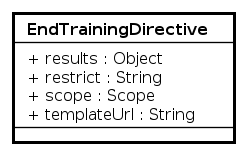
\includegraphics[scale=0.80,keepaspectratio]{UML/Classi/Front-End/QuizziPedia_Front-end_Directives_EndTrainingDirective.png}
			\caption{QuizziPedia::Front-End::Directives::EndTrainingDirective}
		\end{figure} \FloatBarrier
		
		\begin{itemize}
			\item \textbf{Descrizione}: \textit{directive\ped{G}} che permette all'utente di visualizzare il resoconto al termine di un allenamento;
			\item \textbf{Utilizzo}: viene utilizzata per consentire all'utente di visualizzare il resoconto al termine di un allenamento;
			\item \textbf{Relazioni con altre classi}: 
			\begin{itemize}
				\item \textbf{IN \texttt{TrainingView}}: \textit{view\ped{G}} principale per la modalità allenamento;
			\end{itemize}
			\item \textbf{Attributi}:
			\begin{itemize}
				\item \texttt{+ results: Object} \\ oggetto contenente informazioni relative alle risposte date durante l'esercitazione come per esempio il voto e il numero di risposte corrette; 
		\item \texttt{+ restrict: String} \\ Stringa che permette di definire le modalità di inserimento della direttiva all'interno della pagina;
		\item \texttt{+ scope: Scope}: oggetto scope interno della direttiva, contiene le funzionalità per gestire i dati presenti all'interno;
		\item \texttt{+ templateUrl: String} \\ Stringa contenente il percorso del file \textit{HTML\ped{G}} che contiene la direttive.
			\end{itemize}
		\end{itemize}